\documentclass[11pt,a4paper]{article}

\usepackage[margin=1in]{geometry}
\usepackage{hyperref}
\usepackage{enumitem}
\usepackage{booktabs}
\usepackage{listings}
\usepackage{xcolor}
\usepackage{graphicx}
\usepackage{fancyhdr}
\usepackage{titlesec}
\usepackage{tikz}
\usetikzlibrary{shapes.geometric, arrows.meta, positioning, fit, calc}

\hypersetup{
  colorlinks=true,
  linkcolor=blue,
  urlcolor=blue,
}

\lstset{
  basicstyle=\ttfamily\small,
  breaklines=true,
  frame=single,
  backgroundcolor=\color{gray!10},
  keywordstyle=\color{blue},
  commentstyle=\color{green!60!black},
  stringstyle=\color{red!70!black},
}

\pagestyle{fancy}
\fancyhf{}
\rhead{Esusu}
\lhead{Architecture \& Security}
\rfoot{\thepage}

\title{\textbf{Architecture and Security Note}\\[0.5em]
\large Auth, Webhooks, and Data Handling}
\author{Esusu Engineering Team}
\date{\today}

\begin{document}
\maketitle
\tableofcontents
\newpage

%% ============================================================
\section{System Overview}

Esusu is a rotational savings (``esusu'') platform built on:
\begin{itemize}[nosep]
  \item \textbf{Backend:} Next.js 15 App Router (TypeScript), Drizzle ORM, PostgreSQL (Supabase)
  \item \textbf{Payments:} Nomba API (virtual accounts, transfers, webhooks)
  \item \textbf{Frontend:} Next.js with Zustand state management
  \item \textbf{Deployment:} Vercel (serverless functions)
\end{itemize}

The system uses a dedicated Nomba sub-account
(\texttt{49d53c87-e6e4-4c5f-92c6-f13d2579bece}) to scope all payment
operations. Each user receives a unique virtual account (VA) under this
sub-account for collecting contributions.

%% ============================================================
\section{Authentication}

\subsection{Registration Flow}

\begin{enumerate}[nosep]
  \item User submits email, receives a 6-digit OTP via SMTP (Gmail).
  \item OTP is stored in \texttt{otp\_codes} with a 5-minute expiry.
  \item On verification, a bcrypt-hashed password (12 rounds) is saved.
  \item A Nomba virtual account is provisioned under the sub-account for the user.
  \item A JWT is issued and returned to the client.
\end{enumerate}

\subsection{JWT Tokens}

\begin{itemize}[nosep]
  \item \textbf{Algorithm:} HMAC-SHA256 (\texttt{jsonwebtoken} library).
  \item \textbf{Payload:} \texttt{\{ userId, email \}}.
  \item \textbf{Expiry:} Configurable via \texttt{JWT\_EXPIRES\_IN}
        (default \texttt{7d}).
  \item \textbf{Storage:} Client-side (Zustand persist + cookie for
        server-side middleware guard).
\end{itemize}

\subsection{Password Hashing}

\begin{itemize}[nosep]
  \item \textbf{Algorithm:} bcrypt with 12 salt rounds (\texttt{bcryptjs}).
  \item Never stored in plaintext. Verified via \texttt{bcrypt.compare}.
\end{itemize}

\subsection{Account Lockout}

Progressive lockout on failed login attempts:
\begin{table}[h]
  \centering
  \begin{tabular}{cc}
    \toprule
    Failed Attempts & Lockout Duration \\
    \midrule
    5  & 15 minutes \\
    10 & 1 hour \\
    15 & 1 year \\
    \bottomrule
  \end{tabular}
\end{table}

\subsection{Transaction PIN}

A 4-digit PIN (hashed with bcrypt) is required for financial operations
(contributions, withdrawals). Verified via \texttt{/api/v1/auth/verify-pin}.

\subsection{API Route Protection}

All protected routes call \texttt{requireAuth(request)} which:
\begin{enumerate}[nosep]
  \item Extracts the \texttt{Authorization: Bearer <token>} header.
  \item Calls \texttt{verifyToken()} to decode and validate the JWT.
  \item Returns \texttt{401 Unauthorized} if invalid or missing.
\end{enumerate}

There is no Next.js middleware file; auth is enforced at the route handler
level.

%% ============================================================
\section{Webhook Security}

\subsection{Endpoint}

\begin{lstlisting}[language=]
POST /api/v1/webhooks/nomba
\end{lstlisting}

Publicly accessible (no JWT auth required). Security is ensured via HMAC
signature verification.

\subsection{Signature Verification}

Nomba signs every webhook payload using a shared secret
(\texttt{NOMBA\_WEBHOOK\_SECRET}). The verification process:

\begin{enumerate}[nosep]
  \item Construct the signing string by concatenating 9 colon-separated fields:
\begin{lstlisting}
event_type:requestId:userId:walletId:
  transactionId:type:time:responseCode:timestamp
\end{lstlisting}
  \item Compute \texttt{HMAC-SHA256(secret, signing\_string)} and Base64-encode.
  \item Compare with the \texttt{nomba-signature} header using
        \texttt{crypto.timingSafeEqual} (constant-time comparison to
        prevent timing attacks).
  \item Reject with \texttt{401} on mismatch.
\end{enumerate}

\subsection{Timestamp Validation}

\begin{itemize}[nosep]
  \item Parses the \texttt{nomba-timestamp} header (RFC-3339 or epoch ms).
  \item Rejects if the timestamp is older than \textbf{1 hour} (to match
        Nomba's retry window of up to 53 minutes across 5 retries).
  \item Prevents replay attacks from stale payloads.
\end{itemize}

\subsection{Idempotency / Deduplication}

\begin{itemize}[nosep]
  \item Before processing, checks \texttt{webhook\_events} for an existing
        record with the same \texttt{nomba\_request\_id}.
  \item Returns \texttt{"duplicate"} immediately if found (synchronous check).
  \item Inserts the raw payload into \texttt{webhook\_events} with status
        \texttt{"received"} before processing.
\end{itemize}

\subsection{Processing Flow}

\begin{enumerate}[nosep]
  \item Synchronous: signature check $\rightarrow$ timestamp check
        $\rightarrow$ dedup check $\rightarrow$ DB insert $\rightarrow$
        return \texttt{200 Received}.
  \item Asynchronous (fire-and-forget): \texttt{processWebhook()} dispatches
        to the appropriate handler based on \texttt{event\_type}.
  \item Status lifecycle: \texttt{received} $\rightarrow$
        \texttt{processed} / \texttt{failed} / \texttt{unhandled}.
\end{enumerate}

\textbf{Note:} The fire-and-forget pattern means the 200 is returned
immediately. In Vercel serverless, the function may terminate before
processing completes. This is acceptable because the record is already
persisted synchronously.

\subsection{Supported Events}

\begin{table}[h]
  \centering
  \begin{tabular}{ll}
    \toprule
    Event & Action \\
    \midrule
    \texttt{payment\_success}   & Reconcile against contributions \\
    \texttt{payout\_success}    & Mark payout cycle as paid \\
    \texttt{payout\_failed}     & Revert cycle to settling \\
    \texttt{payment\_failed}    & Logged, no action \\
    \texttt{payment\_reversal}  & Logged, no action \\
    \texttt{payout\_refund}     & Logged, no action \\
    \bottomrule
  \end{tabular}
\end{table}

%% ============================================================
\section{Payment Reconciliation}

\subsection{Payment Classification}

Incoming payments are classified based on the ratio of actual vs.\ expected
amount:

\begin{table}[h]
  \centering
  \begin{tabular}{ll}
    \toprule
    Classification & Ratio Range \\
    \midrule
    Exact        & $0.99 \leq r \leq 1.01$ \\
    Underpayment & $0.50 \leq r < 0.99$ \\
    Overpayment  & $1.01 < r \leq 1.50$ \\
    Misdirected  & $r < 0.50$ or $r > 1.50$ \\
    \bottomrule
  \end{tabular}
\end{table}

\subsection{Reconciliation Process}

\begin{enumerate}[nosep]
  \item Match the incoming VA number (\texttt{aliasAccountNumber}) to a
        user's virtual account in the database.
  \item If no match, route to orphan handling.
  \item Look up the user's active circle memberships and expected
        contribution per circle.
  \item Classify the payment and apply accordingly:
    \begin{itemize}[nosep]
      \item \textbf{Exact:} Create a contribution record, update cycle
            totals, check for cycle completion.
      \item \textbf{Underpayment:} Create a partial contribution; the
            remainder becomes a debt.
      \item \textbf{Overpayment:} Apply the expected amount; excess is
            logged and may be credited to the user's wallet.
      \item \textbf{Misdirected:} Flag for manual review.
    \end{itemize}
  \item On cycle completion, trigger payout to the recipient member.
\end{enumerate}

%% ============================================================
\section{Data Handling}

\subsection{Database Schema}

16 PostgreSQL tables managed via Drizzle ORM:

\begin{table}[h]
  \centering
  \small
  \begin{tabular}{ll}
    \toprule
    Table & Purpose \\
    \midrule
    \texttt{users}              & User accounts, credentials \\
    \texttt{circles}            & Savings circles \\
    \texttt{members\_circles}   & Circle membership and rotation order \\
    \texttt{virtual\_accounts}  & Per-user Nomba VAs \\
    \texttt{cycles}             & Individual savings cycles \\
    \texttt{contributions}      & Payment records per member per cycle \\
    \texttt{debts}              & Unpaid/late contribution tracking \\
    \texttt{otp\_codes}         & Email OTPs for registration \\
    \texttt{webhook\_events}    & Raw webhook payloads and processing status \\
    \texttt{wallet\_transactions} & Internal wallet ledger \\
    \texttt{payout\_transactions} & Bank transfer records \\
    \texttt{notifications}      & In-app notifications \\
    \texttt{invite\_codes}      & Circle invitation codes \\
    \texttt{referrals}          & User referral tracking \\
    \texttt{user\_settings}     & Per-user notification preferences \\
    \texttt{contact\_messages}  & Support/contact form submissions \\
    \bottomrule
  \end{tabular}
\end{table}

\subsection{Encryption at Rest}

\begin{itemize}[nosep]
  \item \textbf{Passwords:} bcrypt-hashed (12 rounds). Never stored in
        plaintext.
  \item \textbf{PINs:} bcrypt-hashed. Never stored in plaintext.
  \item \textbf{JWT Secret:} Stored in environment variables, never
        committed to source control.
\end{itemize}

\subsection{Input Validation}

All API endpoints validate required fields and return structured error
responses via the \texttt{ApiResponse} format:

\begin{lstlisting}[language=]
{
  "code": "00" | "01" | "03" | "04" | "05",
  "description": "Success" | "Error message",
  "data": <payload> | null
}
\end{lstlisting}

Response codes:
\begin{itemize}[nosep]
  \item \texttt{00} --- Success
  \item \texttt{01} --- Bad request / validation error
  \item \texttt{03} --- Unauthorized
  \item \texttt{04} --- Not found
  \item \texttt{05} --- Conflict (e.g.\ duplicate)
\end{itemize}

\subsection{Database Connection}

\begin{itemize}[nosep]
  \item Connection pool: max 3 connections, 30s idle timeout, 15s connect
        timeout.
  \item Singleton pattern via \texttt{globalThis} to survive hot reloads
        in development.
  \item All queries use Drizzle ORM (parameterized) --- no raw SQL
        interpolation, preventing SQL injection.
\end{itemize}

\subsection{API Communication with Nomba}

\begin{itemize}[nosep]
  \item Authenticated via OAuth2 client-credentials flow
        (\texttt{POST /v1/auth/token/issue}).
  \item Tokens cached for 55 minutes in memory.
  \item The \texttt{accountId} header always carries the \textbf{parent
        account ID}. The sub-account ID is passed only as a path parameter
        (e.g.\ \texttt{/v1/accounts/virtual/\{subAccountId\}}).
  \item Idempotency keys (\texttt{X-Idempotent-key} header) are used for
        transfer operations to prevent duplicate transactions.
\end{itemize}

%% ============================================================
\section{Security Considerations}

\subsection{Threat Mitigations}

\begin{table}[h]
  \centering
  \small
  \begin{tabular}{lp{7cm}}
    \toprule
    Threat & Mitigation \\
    \midrule
    Webhook forgery     & HMAC-SHA256 signature verification with
                          constant-time comparison \\
    Replay attacks      & 1-hour timestamp window + idempotent dedup via
                          \texttt{nomba\_request\_id} \\
    Brute force login   & Progressive account lockout (5/10/15 attempts) \\
    Password theft      & bcrypt with 12 salt rounds \\
    SQL injection       & Drizzle ORM parameterized queries \\
    Timing attacks      & \texttt{crypto.timingSafeEqual} for signature
                          comparison \\
    Duplicate transfers & Idempotency keys on outbound Nomba API calls \\
    \bottomrule
  \end{tabular}
\end{table}

\subsection{Environment Variables}

Sensitive values are stored in environment variables and never committed:

\begin{table}[h]
  \centering
  \small
  \begin{tabular}{ll}
    \toprule
    Variable & Purpose \\
    \midrule
    \texttt{DATABASE\_URL}            & PostgreSQL connection string \\
    \texttt{JWT\_SECRET}              & HMAC signing key for JWTs \\
    \texttt{JWT\_EXPIRES\_IN}         & Token lifetime \\
    \texttt{NOMBA\_WEBHOOK\_SECRET}   & HMAC key for webhook verification \\
    \texttt{NOMBA\_LIVE\_CLIENT\_ID}  & Nomba API client ID \\
    \texttt{NOMBA\_LIVE\_PRIVATE\_KEY} & Nomba API secret \\
    \texttt{NOMBA\_SUB\_ACCOUNT\_ID}  & Sub-account for scoping VAs \\
    \texttt{SMTP\_USER / SMTP\_PASS}  & Email delivery credentials \\
    \bottomrule
  \end{tabular}
\end{table}

\subsection{Known Limitations}

\begin{enumerate}[nosep]
  \item \textbf{Fire-and-forget webhooks:} Processing runs asynchronously.
        If the Vercel function terminates before \texttt{processWebhook}
        completes, the reconciliation may not execute. Mitigated by the
        synchronous DB insert, which allows manual or cron-based retry.
  \item \textbf{No refresh token rotation:} Refresh tokens use the same
        signing key and expiry as access tokens. A stolen refresh token
        grants long-lived access.
  \item \textbf{OTP whitelist:} Development mode uses a hardcoded phone
        number whitelist with OTP \texttt{999999}. Must be removed before
        production.
  \item \textbf{No rate limiting:} API routes do not enforce rate limits.
        Consider adding middleware for production.
  \item \textbf{No CSRF protection:} JWT is sent via \texttt{Authorization}
        header, which provides some protection, but cookie-based auth
        should include CSRF tokens.
\end{enumerate}

%% ============================================================
\section{Architecture Diagram}

\begin{figure}[h]
\centering
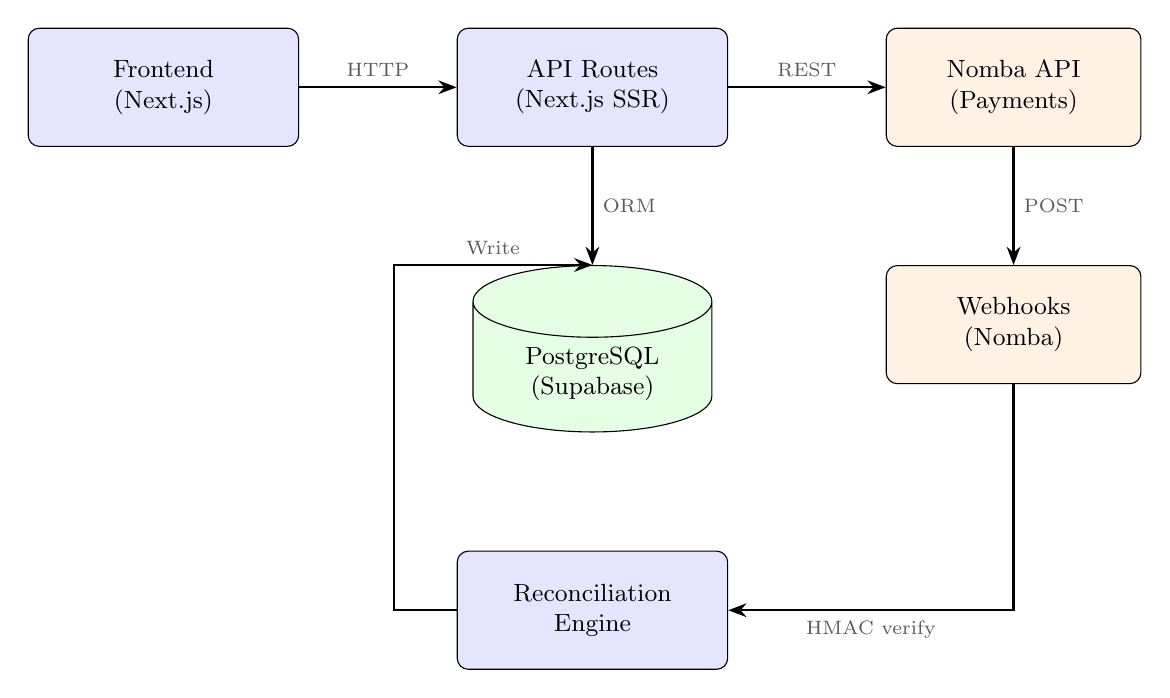
\begin{tikzpicture}[
  block/.style={rectangle, draw, fill=blue!10, text width=3.2cm,
    text centered, rounded corners, minimum height=1.5cm, font=\small},
  dbblock/.style={cylinder, draw, fill=green!10, shape border rotate=90,
    aspect=0.3, text width=2.8cm, text centered, minimum height=1.5cm,
    font=\small},
  extblock/.style={rectangle, draw, fill=orange!10, text width=3cm,
    text centered, rounded corners, minimum height=1.5cm, font=\small},
  arr/.style={-Stealth, thick},
  label/.style={font=\scriptsize, color=gray!70!black}
]

% Nodes
\node[block] (fe) {Frontend\\(Next.js)};
\node[block, right=2cm of fe] (api) {API Routes\\(Next.js SSR)};
\node[extblock, right=2cm of api] (nomba) {Nomba API\\(Payments)};
\node[dbblock, below=1.5cm of api] (db) {PostgreSQL\\(Supabase)};
\node[extblock, below=1.5cm of nomba] (wh) {Webhooks\\(Nomba)};
\node[block, below=1.5cm of db] (recon) {Reconciliation\\Engine};

% Arrows
\draw[arr] (fe) -- node[above, label] {HTTP} (api);
\draw[arr] (api) -- node[above, label] {REST} (nomba);
\draw[arr] (api) -- node[right, label] {ORM} (db);
\draw[arr] (nomba) -- node[right, label] {POST} (wh);
\draw[arr] (wh.south) |- node[near end, below, label] {HMAC verify} (recon.east);
\draw[arr] (recon.west) -- ++(-0.8,0) |- node[near end, above, label] {Write} (db.north);

\end{tikzpicture}
\caption{System architecture showing the request flow from frontend through API to Nomba, with webhook-based reconciliation loop.}
\end{figure}

%% ============================================================
\section{Conclusion}

The Esusu platform implements defense-in-depth across authentication,
webhook processing, and data handling. Key security properties:
\begin{itemize}[nosep]
  \item All sensitive data (passwords, PINs) is hashed at rest.
  \item Webhook authenticity is verified via HMAC-SHA256 with
        constant-time comparison.
  \item Financial operations require both JWT authentication and PIN
        verification.
  \item Idempotency is enforced at both the webhook ingestion layer and
        outbound Nomba API calls.
\end{itemize}

\end{document}
